\bibliographystyle{babplain-fl}

% To do:
% - Check programs

\chapter{Quicksort}
\label{cha:quicksort}

  Quicksort,
  debido a Hoare~\cite{hoare62:_quicksort},
  es otro algoritmo basado en dividir y conquistar,
  pero en este caso la división no es fija.
  Referencia obligatoria es el detallado análisis de Sedgewick~%
    \cite{sedgewick77:_analysis_quicksort}.
  Dado un rango de elementos de un arreglo a ser ordenado,
  se elige un elemento \emph{pivote} de entre ellos
  y se reorganizan los elementos en el rango
  de forma que todos los elementos menores que el pivote
  queden antes de los mayores que éste.
  \begin{figure}[htbp]
    \centering
    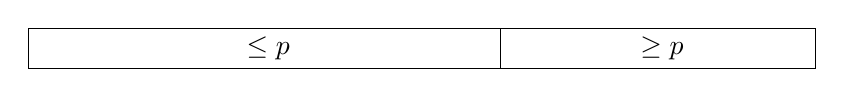
\begin{tikzpicture}
      \draw (0, 0) rectangle (6, 0.5) node [pos = 0.5] {\({} \le p\)};
      \draw (6, 0) rectangle (10, 0.5) node [pos = 0.5] {\({} \ge p\)};
    \end{tikzpicture}
    \caption{Idea de Quicksort}
    \label{fig:qsort:idea}
  \end{figure}
  Con esto bastará ordenar recursivamente cada uno
  de los dos nuevos rangos generados
  para completar el trabajo.
  \begin{figure}[htbp]
    \centering
    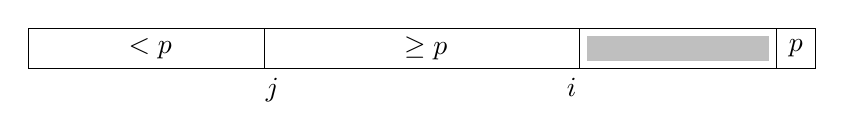
\begin{tikzpicture}
      \draw ( 0,  0) rectangle ( 3,   0.5) node [pos = 0.5] {\({} < p\)};
      \draw ( 3,   0) rectangle ( 7,   0.5) node [pos = 0.5] {\({} \ge p\)};
      \draw ( 7,   0) rectangle ( 9.5, 0.5);
      \draw [fill = lightgray, lightgray] (7.1, 0.1) rectangle (9.4, 0.4);
      \draw ( 9.5, 0) rectangle (10,   0.5) node [pos = 0.5] {\(p\)};
      \node at (3.1, 0) [below] {\(j\)};
      \node at (6.9, 0) [below] {\(i\)};
    \end{tikzpicture}
    \caption{Particionamiento de Lomuto}
    \label{fig:qsort:Lomuto}
  \end{figure}
  La figura~\ref{fig:qsort:Lomuto}
  esquematiza una manera popular de explicar esta \emph{partición}:
  se elige un pivote de forma aleatoria
  y el pivote elegido se intercambia con el último elemento del rango
  (para sacarlo de en medio).
  En un ciclo se revisa el rango,
  elementos menores que el pivote
  se intercambian con el primero que se sabe mayor.
  \lstinputlisting[float,
                   language=C,
                   firstline = 23, lastline = 37,
                   caption={Versión simple de Quicksort
                            (particionamiento de Lomuto)},
                   label=lst:quicksort-Lomuto]
                   {code/quicksort-0.c}
% LaTeX bug: Leaving out the "float, ..." line gives a crash
  El ciclo de particionamiento mantiene el invariante
  que los elementos en el rango \(m\) a~\(j\) (exclusive)
  son menores que el pivote,
  los entre \(j\) (inclusive) a \(i\) son mayores o iguales al pivote,
  y el resto aún sin clasificar.
  Este algoritmo se atribuye a Lomuto,
  fue popularizado por Bentley~%
    \cite{bentley99:_programming_pearls}.
  El listado~\ref{lst:quicksort-Lomuto}
  muestra una versión simple del programa,
  que elige siempre el último elemento del rango como pivote.

  El esquema original de Hoare es mucho más eficiente,
  pero también notoriamente sutil
  (Bentley~%
    \cite{bentley07:_most_beaut_code_i_never_wrote}
   reconoce que nunca lo entendió del todo,
   a pesar de usarlo por años).
  Elige un pivote en el rango
  (en nuestra versión simple elegimos el elemento del medio),
  luego busca un elemento mayor al pivote desde la izquierda
  y uno menor desde la derecha.
  Si los índices no se han cruzado,
  están en el tramo equivocado y se intercambian.
  No es obvio que con el código indicado
  los índices nunca salen del rango dado.
  Tampoco conocemos la posición final del pivote,
  solo sabemos que los elementos hasta el índice \((j\) (inclusive)
  son menores o iguales que éste.
  El listado~\ref{lst:quicksort-Hoare}
  da detalles.
  \lstinputlisting[float,
                   language=C,
                   firstline = 23, lastline = 38,
                   caption={Versión simple de Quicksort
                            (particionamiento de Hoare)},
                   label=lst:quicksort-Hoare]
                   {code/quicksort-1.c}

\section{Análisis del promedio}
\label{sec:promedio-qsort}

  Evaluaremos el tiempo promedio de ejecución del algoritmo.
  Supondremos~\(n\) elementos todos diferentes,
  que las \(n!\)~permutaciones de los \(n\)~elementos
  son igualmente probables,
  y que el pivote se elige al azar en cada etapa.
  En este caso está claro que el método de particionamiento planteado
  no altera el orden de los elementos en las particiones
  respecto del orden que tenían originalmente.
  Luego,
  los elementos en cada partición también son una permutación al azar.

  Para efectos del análisis del algoritmo
  tomaremos como medida de costo el número promedio de comparaciones
  que efectúa Quicksort al ordenar un arreglo de \(n\)~elementos.
  El trabajo adicional que se hace en cada partición
  será aproximadamente proporcional a esto,
  por lo que esta es una buena vara de medida.
  Al particionar,
  cada uno de los \(n - 1\) elementos fuera del pivote
  se comparan con este exactamente una vez en el método planteado,
  y además es obvio que este es el mínimo número de comparaciones necesario
  para hacer este trabajo.
  Si llamamos \(k\) a la posición final del pivote,
  el costo de las llamadas recursivas que completan el ordenamiento
  será \(C(k - 1) + C(n - k)\).
  Si elegimos el pivote al azar
  la probabilidad de que \(k\) tenga un valor cualquiera entre~\num{1}
  y~\(n\) es la misma.
  Cuando el rango es vacío no se efectúan comparaciones.
  Estas consideraciones llevan a la recurrencia:
  \begin{equation*}
    C(n)
       =  n - 1 +
           \frac{1}{n} \, \sum_{1 \le k \le n}
              \left(C(k - 1) + C(n - k)\right) \quad C(0)  = 0
  \end{equation*}
  Por simetría podemos simplificar la suma,
  dado que estamos sumando los mismos términos
  en orden creciente y decreciente.
  Extendiendo el rango de la suma y multiplicando por \(n\) queda:
  \begin{equation*}
    n C(n)
      = n (n - 1) + 2 \sum_{0 \le k \le n - 1} C(k)
  \end{equation*}
  Ajustando los índices:
  \begin{equation*}
    (n + 1) C(n + 1)
      = n (n + 1) + 2 \sum_{0 \le k \le n} C(k) \quad C(0) = 0
  \end{equation*}

  Definimos la función generatriz ordinaria:
  \begin{equation*}
    c(z)
      = \sum_{n \ge 0} C(n) z^n
  \end{equation*}
  Aplicando las propiedades de funciones generatrices ordinarias
  a la recurrencia
  queda la ecuación diferencial:
  \begin{align*}
    \left( z \mathrm{D} + 1 \right) \, \frac{c(z)}{z}
      &= \left( (z \mathrm{D})^2 + z D \right) \, \frac{1}{1 - z}
           + \frac{2 c(z)}{1 - z}
           \qquad c(0) = 0 \\
    c'(z)
      &= \frac{2 c(z)}{1 - z} + \frac{2 z}{(1 - z)^3}
  \end{align*}
  La solución a esta ecuación es:
  \begin{equation*}
    c(z)
      = - 2 \, \frac{\ln (1 - z)}{(1 - z)^2}
            - \frac{2 z}{(1 - z)^2}
  \end{equation*}
  El primer término corresponde
  a la suma parcial de números harmónicos
  (se deriva su función generatriz
   en~\cite[capítulo 19]{brand17:_fundamentos_informatica}),
  el segundo término da un coeficiente binomial:
  \begin{align*}
    C(n)
      &= 2 \sum_{0 \le k \le n} H_k - 2 \, \binom{n}{1} \\
      &= 2 \sum_{0 \le k \le n} H_k - 2 n
  \end{align*}
  Para el primer término,
  consideremos cuántas veces aparece \(1/k\) en la suma:
  \begin{align}
    \sum_{0 \le k \le n} H_k
      &= \sum_{0 \le k \le n} \sum_{1 \le r \le k} \frac{1}{r} \notag \\
      &= \sum_{1 \le r \le n} \frac{n - r + 1}{r} \notag \\
      &= (n + 1) \sum_{1 \le r \le n} \frac{1}{r} - n
            \label{eq:Hn-sum}
  \end{align}
  Otra opción
  es sumar por partes
  (ver el apunte de Fundamentos de Informática,
   ecuación~(1.34)).
  Esto da finalmente:
  \begin{equation}
    \label{eq:quicksort-comparisons}
    C(n)
      = 2 (n + 1) H_n - 4 n
  \end{equation}
  Sabemos que
  (ver~\cite[capítulo 18]{brand17:_fundamentos_informatica})
  que \(H_n = \ln n + \gamma + O(1 / n)\),
  donde \(\gamma = 0,57721\,56649\,01532\,65120\)
  con lo que \(C(n) = 2 n \ln n + O(n)\).

\section{Análisis del peor y mejor caso}
\label{sec:peor-mejor-qsort}

  Pero podemos hacer más.
  En el peor caso,
  al particionar en cada paso elegimos uno de los elementos extremos,
  con lo que las particiones son de largo 0 y \(n - 1\),
  lo que da lugar a la recurrencia:
  \begin{equation*}
    C_{\text{peor}}(n)
      = n - 1 + C_{\text{peor}}(n - 1) \quad C_{\text{peor}}(0) = 0
  \end{equation*}
  Las técnicas estándar dan como solución:
  \begin{align*}
    C_{\text{peor}}(n)
      &= \frac{n (n - 1)}{2} \\
      &= \frac{1}{2} n^2 + O(n)
  \end{align*}
  El mejor caso es cuando en cada paso la división es equitativa,
  lo que lleva casi a la situación de dividir y conquistar
  analizada antes
  con \(a = 2\), \(b = 2\) y \(d = 1\),
  cuya solución sabemos es \(C_{\text{mejor}}(n) = O(n \log n)\).
  Un análisis más detallado,
  restringido al caso en que \(n = 2^k - 1\)
  de manera que los dos rangos siempre resulten del mismo largo,
  es como sigue.
  La recurrencia original se reduce a:
  \begin{equation*}
    C_{\text{mejor}}(n)
      = n - 1 + 2 C_{\text{mejor}}((n - 1) / 2)
      \quad C_{\text{mejor}}(0) = 0
  \end{equation*}
  Con el cambio de variables:
  \begin{equation*}
    n = 2^k - 1 \quad F(k) = C_{\text{mejor}}(2^k - 1)
  \end{equation*}
  esto se transforma en:
  \begin{equation*}
    F(k)
      = 2^k - 2 + 2 F(k - 1) \quad F(0) = 0
  \end{equation*}
  cuya solución es:
  \begin{align*}
    F(k)
      &= k 2^k + 2^{k + 1} + 2 \\
    C_{\text{mejor}}(n)
      &= (n + 1) \log_2 (n + 1) + 2 (n + 1) + 2 \\
      &= \frac{1}{\ln 2} \, n \ln n + O(n)
  \end{align*}
  La constante en este caso es aproximadamente \num{1,443},
  el mejor caso no es demasiado mejor que el promedio;
  pero el peor caso es mucho peor.

\section{Consideraciones prácticas}
\label{sec:consideraciones-practicas}

  Una variante común
  es usar un método de ordenamiento simple para rangos chicos,
  dado que Quicksort es más costoso que métodos simples para rangos pequeños.
  Una opción es cortar la recursión
  no cuando el rango se reduce a un único elemento
  sino cuando cae bajo un cierto margen;
  y luego se ordena todo mediante inserción,
  que funciona muy bien si los datos vienen \textquote{casi ordenados},
  como resulta de lo anterior.
  Para analizar esto se requieren medidas más ajustadas
  del costo de los métodos,
  y se cambian las condiciones de forma que para valores de \(n\)
  menor que el límite se usa el costo del método alternativo.
  Esto puede hacerse,
  pero es bastante engorroso y no lo veremos acá.

  Para evitar el peor caso
  (que se da cuando el pivote es uno de los elementos extremos)
  una opción es tomar una muestra de elementos y usar la mediana
  (el elemento del medio de la muestra)
  como pivote.
  La forma más simple de hacer esto es tomar tres elementos.
  Como además es frecuente que se invoque el procedimiento con un arreglo
  \textquote{casi ordenado}
  (o incluso ya ordenado),
  conviene tomar como muestra el primero,
  el último
  y un elemento del centro,
  de forma de elegir un buen pivote incluso en ese caso patológico.
  A esta idea se le conoce como \emph{mediana de tres}.
  Esta estrategia disminuye un tanto la constante
  por efecto de una división más equitativa.
  Tiene la ventaja adicional
  que tener elementos menor que el pivote al comienzo del rango
  y mayor al final
  no es necesario comparar índices para determinar
  si se llegó al borde del rango.
  El análisis detallado se encuentra por ejemplo en Sedgewick y Flajolet~%
    \cite{sedgewick13:_introd_anal_algor}.

  Por el otro lado,
  McIllroy~\cite{mcillroy99:_killer_adver_quicksort}
  muestra cómo lograr que siempre tome el máximo tiempo posible.
  Quicksort
  (haciendo honor a su nombre)
  es muy rápido
  ya que las operaciones en sus ciclos internos
  implican únicamente una comparación
  y un incremento o decremento de un índice.
  Es ampliamente usado,
  y como su peor caso es muy malo,
  vale la pena hacer un estudio detallado de la ingeniería del algoritmo,
  como hacen Bentley y McIllroy~%
    \cite{bentley93:_engin_sort_funct}.
  Debe tenerse cuidado con Quicksort por su peor caso,
  si un atacante puede determinar los datos
  puede hacer que el algoritmo consuma muchísimos recursos.
  Para evitar el peor caso se ha propuesto cambiar a Heapsort,
  debido a Williams~%
    \cite{williams64:_alg_heapsort}
  (garantizadamente \(O(n \log n)\),
   pero mucho más lento que Quicksort)
  si se detecta un caso malo,
  como propone Musser~\cite{musser97:_introsort}.

  Lo anterior supone que todos los valores son diferentes.
  Si hay muchos elementos repetidos
  (en el extremo,
   son todos iguales),
  resulta que si al particionar pasamos elementos iguales al pivote
  caemos en el peor caso
  (el pivote termina en un extremo).
  Conviene parar si hallamos un elemento igual al pivote,
  como se hace en el listado~\ref{lst:quicksort-Hoare}.

  Pero lo que realmente nos conviene es particionar en \emph{tres} tramos,
  como muestra la figura~\ref{fig:fat-partition}.
  \begin{figure}[htbp]
    \centering
    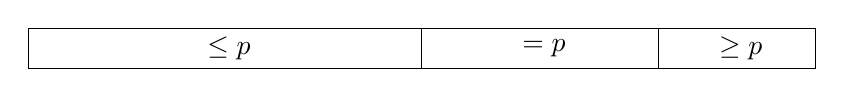
\begin{tikzpicture}
      \draw (0, 0) rectangle ( 5, 0.5) node [pos = 0.5] {\({} \le p\)};
      \draw (5, 0) rectangle ( 8, 0.5) node [pos = 0.5] {\({} = p\)};
      \draw (8, 0) rectangle (10, 0.5) node [pos = 0.5] {\({} \ge p\)};
    \end{tikzpicture}
    \caption{Particionamiento ancho}
    \label{fig:fat-partition}
  \end{figure}
  Esto es una variante del \emph{problema de la bandera holandesa}
  (\emph{\foreignlanguage{english}{Dutch national flag problem}},
   ver la figura~\ref{fig:dutch-flag})
  propuesto por Dijkstra~%
    \cite{dijkstra76:_discipline_programming}:
  dada una secuencia de canicas de colores rojo, blanco y azul,
  ordenarlas de manera de tener juntas las rojas, las blancas y las azules.
  \begin{figure}[ht]
    \centering
    
\begin{tikzpicture}
      \draw (0, 0) [fill = blue] rectangle (4.5, 1);
      \draw (0, 1)		 rectangle (4.5, 2);
      \draw (0, 2) [fill = red]	 rectangle (4.5, 3);
    \end{tikzpicture}
    \caption{La bandera holandesa}
    \label{fig:dutch-flag}
  \end{figure}
  Una manera de efectuar esto
  es usar el invariante de la figura~\ref{fig:fat-partition-invariant}.
  \begin{figure}[ht]
    \centering
    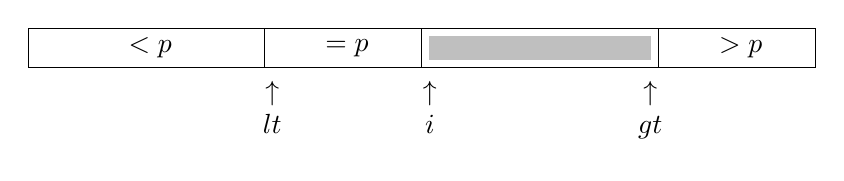
\begin{tikzpicture}
      \draw (0, 0) rectangle ( 3, 0.5) node [pos = 0.5] {\({} < p\)};
      \draw (3, 0) rectangle ( 5, 0.5) node [pos = 0.5] {\({} = p\)};
      \draw (5, 0) rectangle ( 8, 0.5);
      \draw [fill = lightgray, lightgray] (5.1, 0.1) rectangle (7.9, 0.4);
      \draw (8, 0) rectangle (10, 0.5) node [pos = 0.5] {\({} > p\)};
      \node at (3.1, 0) [below]
         {\(\begin{array}{c} \uparrow \\ \text{lt} \end{array}\)};
      \node at (5.1, 0) [below]
         {\(\begin{array}{c} \uparrow \\ \text{i} \end{array}\)};
      \node at (7.9, 0) [below]
         {\(\begin{array}{c} \uparrow \\ \text{gt} \end{array}\)};
    \end{tikzpicture}
    \caption{Invariante para particionamiento ancho}
    \label{fig:fat-partition-invariant}
  \end{figure}
  Código es como indica el listado~\ref{lst:particion-2}.
  \lstinputlisting[float = ht,
                   language=C,
                   caption={Partición ancha},
                   label=lst:particion-2]
                   {code/partition-2.c}

  Durante mucho tiempo se consideró poco práctico
  Quicksort con más de un pivote,
  hasta que en 2009 se adoptó una variante con dos pivotes en Java~7,
  el algoritmo de Yaroslavskiy, Bentley y Bloch~%
    \cite{yaroslavskiy09:_dual_pivot_quick_algor}.
  Desde entonces se han analizando opciones con más de un pivote,
  una selección de referencias recientes es~%
    \cite{aumueller16:_how_good_multi_pivot_quicksort,
          kushagra14:_multi_pivot_quicksort}.
  Resulta que su mejor rendimiento se debe a efectos de memoria caché.
% To do: Show model, solution...

% To do:
% - Program(s) integrating all proposals

\bibliography{../referencias}

%%% Local Variables:
%%% mode: latex
%%% TeX-master: "../INF-221_notas"
%%% ispell-local-dictionary: "spanish"
%%% End:

% LocalWords:  Quicksort Particionamiento particionamiento Heapsort
% LocalWords:  particionar garantizadamente english Dutch national
% LocalWords:  flag problem
